\hypertarget{agile-estimating-and-planning}{%
\section{Agile Estimating and
Planning}\label{agile-estimating-and-planning}}

Ensures that we are on the right path. In Scrum you plan a lot. You plan every daily standup meeting. You estimate the work every week. A scrum team has several plans, the coarse and fine grained plans for weeks and months. Organization needs planning!
A good iterative planning process:

\begin{itemize}
\tightlist
\item
  Reduces risk
\item
  Reduces uncertainty
\item
  Supports better decision making
\item
  Establishes trust
\item
  Conveys information
\end{itemize}

\begin{itemize}
\tightlist
\tightlist
\item
  Agile planning shifts the emphasis from the plan to the planning!
\item
  Agile plans are often changed during a projects and that's good!
\item
  Key idea: A project rapidly and reliably generates a flow of useful
  new capabilities and new knowledge
\end{itemize}

\begin{figure}[H]
\centering
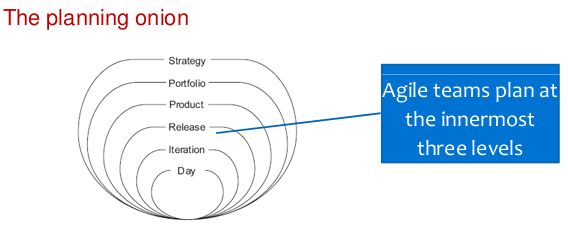
\includegraphics[width=0.5\textwidth]{figures/planningOnion.png}
\caption{Planning Onion}
\end{figure}

\hypertarget{estimating-with-story-points}{%
\subsection{Estimating with Story
Points}\label{estimating-with-story-points}}

\begin{itemize}
\tightlist
\item
  Story points are a relative measure of the complexity of a user story
\item
  Velocity is a measure of a team's rate of progress per iteration
\item
  The duration of a project is not estimated as much as it is derived by
  taking the total number of story points and dividing it by the
  velocity of the team
\item
  Ideal time and elapsed time are different
  \subitem \textbf{Ideal Time :} Time without peripheric activities. (football game $\rightarrow$ 90 min)
  \subitem \textbf{Elapsed Time :} Estimated time (football game $\rightarrow$ 4 hrs)
\end{itemize}


\hypertarget{techniques-for-estimating}{%
\subsubsection{Techniques for
estimating}\label{techniques-for-estimating}}

\begin{itemize}
\tightlist
\item
  At some point, it doesn't make sense to put more effort into the
  estimation, because the results are getting worse.
\item
  Estimates are best derived collaboratively by the team play Planning
  Poker
\item
  Two possible estimation scales (10x range):

  \begin{itemize}
  \tightlist
  \item
    Fibonacci: 1,2,3,5, and 8
  \item
    2\^{}n: 1,2,4, and 8
  \end{itemize}
  
  \item Use a referency story where you can esitimate relativiely from.
\end{itemize}

\hypertarget{user-stories-epics-and-themes}{%
\subsubsection{User Stories, Epics, and
Themes}\label{user-stories-epics-and-themes}}

\begin{itemize}
\tightlist
  \item \textbf{A Userstory} describes Who, What and why from the perspective of the user.
\item
  Fine-grained level: User Story (10x range)
\item
  A large user story is called an \textbf{epic}
\item
  A set of related user stories may be combined and treated as a single
  entity. This is referred to as a \textbf{theme}
\item
  Estimation scale for epics and themes can be higher up to 100
\end{itemize}

\hypertarget{release-plan}{%
\subsection{Release Plan}\label{release-plan}}

\begin{itemize}
\tightlist
\item
  Release date (three to nine months)
\item
  Prioritized list of user stories with there estimates
\item
  Number and length of iterations
\item
  Product owner's conditions of satisfaction
\item
  Estimated velocity
\item
  The release plan is updated at the start of each iteration
\end{itemize}

\hypertarget{planning-poker}{%
\subsubsection{Planning Poker}\label{planning-poker}}

\begin{itemize}
\tightlist
\item
  Each estimator is given a deck of cards, each card has a valid
  estimate written on it
\item
  Customer/Product owner reads a story and it's discussed briefly
\item
  Each estimator selects a card that's his or her estimate
\item
  Cards are turned over so all can see them
\item
  Discuss differences (especially outliers)
\item
  Re-estimate until estimates converge
\end{itemize}

\hypertarget{conditions-of-satisfaction}{%
\subsubsection{Conditions of
Satisfaction}\label{conditions-of-satisfaction}}

\begin{itemize}
\tightlist
\item
  Before starting to plan a release, it is important to know the
  \textbf{criteria} by which the project will be evaluated as a
  \textbf{success} or a \textbf{failure}
\item
  Leading indicators are usually: schedule, scope and resources
\item
  The product owner conditions of satisfactions are defined by a
  combination of schedule, scope and resource goals
\item
  A \textbf{date-driven project} is one that must be released by a
  certain date but for which the feature set is negotiable
\item
  A \textbf{feature-driven project} is one for which we consider the
  completion of a set of features to be more important
\end{itemize}

\hypertarget{iteration-length}{%
\subsubsection{Iteration length}\label{iteration-length}}

\begin{itemize}
\tightlist
\item
  Most of the teams work with iterations from \textbf{two or four weeks}
\item
  Factors afferting the iteration length are:

  \begin{itemize}
  \tightlist
  \item
    The length of the release being worked on
  \item
    The amount of uncertainty
  \item
    The ease of getting feedback
  \item
    How long priorities can remain unchanged
  \item
    Willingness to go without feedback
  \item
    The overhead of iterating
  \item
    A feeling of urgency is maintained
  \end{itemize}
\end{itemize}

\hypertarget{priorization}{%
\subsubsection{Priorization}\label{priorization}}

\begin{itemize}
\tightlist
\item
  For the priorization of the user stories, the product owner defines a
  list of acceptance thresholds which is a simple classification of what
  the importance levels in the product backlog actually mean in terms of
  the contract.
\item
  These thresholds can then be helpful and be classified

  \begin{itemize}
  \tightlist
  \item
    e.g.~All items with importance \textgreater{}= 100 must be included
    in version 1.0, or else we'll be fined to death.
  \end{itemize}
\end{itemize}

\hypertarget{iteration-planning}{%
\subsection{Iteration Planning}\label{iteration-planning}}

\begin{itemize}
\tightlist
\item
  Unlike a release plan, an iteration plan looks in more detail at the
  specific work of a single iteration.
\item
  Rather than the three to nine month horizon of a typical release plan,
  the iteration plan looks out no further than a single iteration.
\item
  The fairly large user stories of a release plan are decomposed into
  tasks on the iteration plan.
\item
  Each task is estimated in terms of the number of ideal hours the task
  will take to complete.
\end{itemize}

\hypertarget{values-for-planning}{%
\subsubsection{Values for planning}\label{values-for-planning}}

\begin{itemize}
\tightlist
\item
  Which features should be developed?
\item
  Factors in Prioritization of the User Stories
\item
  The financial value of having the features

  \begin{itemize}
  \tightlist
  \item
    e.g.~Amount of money earned or saved
  \item
    ``Prioritize on business value''; how much money will the
    organization make or save by having the new feature
  \item
    Internal Rate of Return (IRR and sometimes called Return On
    Investment or ROI)
  \end{itemize}
\item
  The cost of developing (and supporting) the new features

  \begin{itemize}
  \tightlist
  \item
    How many Story Points?
  \end{itemize}
\item
  The amount and significance of learning and new knowledge created by
  developing the features
\item
  The amount of risk removed by developing the features
\end{itemize}

\hypertarget{new-knowledge}{%
\subsubsection{New Knowledge}\label{new-knowledge}}

\begin{itemize}
\tightlist
\item
  On many projects, much of the the overall effort is spent in the
  pursuit of new knowledge.
\item
  It is important that this effort be acknowledged and considered
  fundamental to the project: At the start of a project we never know
  everything that we'll need to know by the end of the project.

  \begin{itemize}
  \tightlist
  \item
    Knowledge about the product (What will be developed)
  \item
    Knowledge about the project (How the product will be created)
  \end{itemize}
\end{itemize}




\clearpage